\chapter{\label{chap:szenarien}Szenarien}
Alle in Kapitel \ref{chap:state} angeführten Technologien haben die Unterstützung der Erstellung von offlinefähigen Anwendungen gemeinsam.
Prinzipiell sollte eine Offline First Anwendung in der Lage sein, mit fehlender Internetverbindung zu funktionieren und mit auftretenden Konflikten so umgehen zu können, dass keine Daten verloren gehen.
Sie muss die Fälle behandeln können, die sich aus den folgenden Szenarien ergeben.
Dafür werden zunächst Szenarien in der \todo{Netzwerkübetragung als `Voraussetzung für die der Konfliktentstehung`} aufgezeigt.
%
%
% Netzwerk Szanarien (fail)   ------------------------------------------------------------------------------------------------------------------------------------------------
%
\section{\label{sec:netszenarien}Szenarien bei der Datenübertragung}
Im einfachen Anwendungsbeispiel einer Kontaktliste gibt es zwei Parteien die miteinander interagieren: die Liste als Client und den Server. Folgende Situationen können bei der Übertragung von Daten über das Netzwerk eintreten.
\begin{figure}[H]
  \centering
  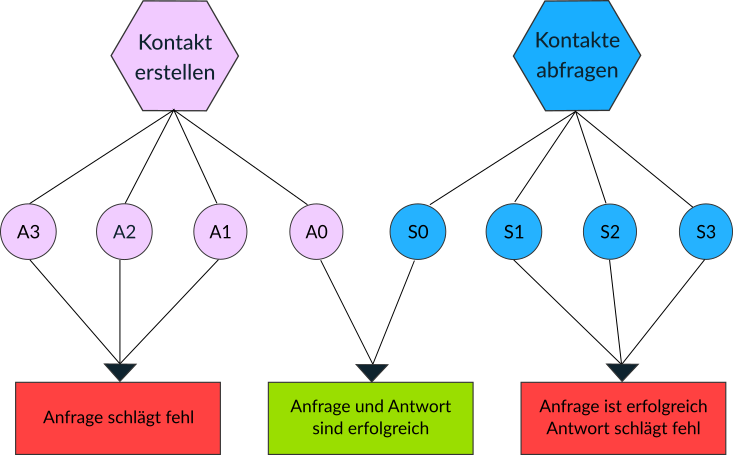
\includegraphics[width=0.8\textwidth]{Szenarien}
  \grayRule
  \caption{Szenarien bei der Datenübertragung über das Netzwerk}
  \label{fig:szenarien}
\end{figure}
\todo{Erstellen = erstellen, aktualisieren, löschen}
\begin{description}[leftmargin=0.5cm,style=nextline]
% client push
\item[Szenario A0:]
Der Client erstellt einen Adressbucheintrag, hat den Status \sc{online} und der Server ist erreichbar. Sowohl Anfrage als auch Antwort ist erfolgreich. Der Kontakt wird erfolgreich erstellt.\\
\item[Szenario A1:]
Der Client erstellt einen Adressbucheintrag, hat den Status \sc{offline} und der Server ist nicht erreichbar. Die Anfrage schlägt fehl.\\
\item[Szenario A2:]
Der Client erstellt einen Adressbucheintrag und hat den Status \sc{online}. Die Anfrage wird gestartet und währenddessen bricht die Internetverbindung ab. Die Anfrage `wartet` bis ein Timeout getriggert wird und schlägt dann fehl. Wärend des Wartens ist der Client blockiert.\\
\item[Szenario A3:]
Der Client erstellt einen Adressbucheintrag und hat den Status \sc{online}. Die Anfrage wird gestartet und währenddessen bricht die Internetverbindung ab. Die Anfrage ist teilweise erfolgreich. Nur ein Teil der Telefonnummer kommen beim Server an.\\
% client pull / server push
\item[Szenario S0:]
Der Client fordert eine Liste aller gespeicherten Kontakte vom Server an, hat den Status \sc{online} und der Server ist erreichbar. Sowohl Anfrage als auch Antwort ist erfolgreich. Die Liste wird komplett ausgeliefert.\\
\item[Szenario S1:]
Der Client fordert eine Liste aller gespeicherten Kontakte vom Server an, hat den Status \sc{offline} und der Server ist nicht erreichbar. Die Antwort schlägt fehl.\\
\item[Szenario S2:]
Der Client fordert eine Liste aller gespeicherten Kontakte vom Server an und hat den Status \sc{online}. Während der Server antwortet bricht die Internetverbindung ab. Die Antwort `wartet` bis ein Timeout getriggert wird schlägt dann fehl. Wärend des Wartens ist der Client blockiert.\\
\item[Szenario S3:]
Der Client fordert eine Liste aller gespeicherten Kontakte vom Server an und hat den Status \sc{online}. Während der Server antwortet bricht die Internetverbindung ab. Die Antwort ist teilweise erfolgreich. Nur ein Teil der angefragten Daten kommen beim Client an.
\end{description}
In den obigen Szenarien wird nicht beschrieben warum die Internetverbindung abbricht. Dies kann verschiedene Gründe haben. Um nur einige Beispiele zu nennen: Eine langsame Internetverbindung, oder eine Fahrt durch einen Tunnel kann ein Timeout während einer Aktion hervorrufen. Ein auf einer Baustelle gekapptes Kabel oder ein Stromausfall kann zu zeitweise vollständigen Internetverlust (haha) führen.
%
% ERGEBNIS
%
\subsubsection*{Ergebnis}
Da die Szenarien \it{A0} und \it{S0}, die Szenarien \it{A1}, \it{A2} und \it{A3} sowie die Szenazien \it{S1}, \it{S2} und \it{S3} zusammengefasst werden können, ergeben sich aus den acht Szenarien die drei nun aufgezählten Fälle.
\begin{itemize}
  \item Fall a: Anfrage und Antwort sind erfolgreich.
  \item Fall b: Anfrage ist nicht erfolgreich
  \item Fall c: Anfrage ist erfolgreich, Antwort schlägt fehl
\end{itemize}
%\todo{Bezug auf die Netzwerkfails. Wenn die Anfrage fehlschlägt, kann man das im Client gut lösen (im Hintergrund (in intervallen) nochmal senden..) Oder das erst am Ende?}
Von den erarbeiteten Fällen sind Fall \it{b} und \it{c} für die Szenarien zur Konfliktentstehung relevant: Die Anfrage oder die Antwort schlägt fehl.
%
%
% Konflikte   ----------------------------------------------------------------------------------------------------------------------------------------------------------------------------
%
\section{\label{sec:konfliktszenarien}Szenarien zur Konfliktentstehung}
Im Anwendungsbeispiel einer Kontaktliste können mehrere Personen die Liste verwalten. Die Komplexität wird durch mehr Parteien -- beliebig viele Clients -- erhöht.
Jede Person kann alle Einträge jederzeit laden und einzelne erstellen, bearbeiten oder löschen. Bei den Ausführungen der grundlegenden \gls{CRUD} Operarionen kann es bei der Synchronisation der beteiligten Parteien zu Konflikten kommen wenn einer der oben genannten Fälle (\it{b,c}) eintritt und ein Objekt von mehreren Parteien bearbeitet wird.
Für die effiziente Nutzung der Anwendung sollen bei jedem Start der Anwendung nur die neuen und die gegebenenfalls aktualisierten Einträge geladen werden. Alle Adressbucheinträge müssen identifiziert und versioniert werden. Folgende Situationen können eintreten:
% \highlight{Damit die Einträge sortiert und gefiltert aus der Datenbank geladen werden können, werden sie mit einem Index versehen. Jeder neue Eintrag bekommt automatisch einen höheren Index. Die aktualisierten Objekte sollen ebenfalls geladen werden, aber keinen neuen Index bekommen. Deswegen gibt es neben dem Datensatz \sc{Adressbucheinträge} zusätzlich den der \sc{Aktualisierungen} mit einem sich automatisch erhöhendem Index \it{und der Referenz zum Adressbucheintrag}. \todo{eigenes Szenario?}. Mit jeder Aktualisierung oder Löschung eines Kontakts wird im Aktualisierungsdatensatz der Index durch einen neuen ersetzt. So hat jede Kontakt-ID eine Aktualisierungs-ID und ein Eintrag wird auch nach mehrmaligem Aktualisieren nicht mehrfach geladen.}\\
%
%
% Footnotes
%
\def \naturalkey {Ein Schlüssel, der sich aus einem Attribut des Objekts ergibt oder sich aus mehreren Attributen zusammensetzt. So könnte ein sprechender Schlüssel von Jean-Luc Picard mit der E-Mail-Adresse picard@enterpise.com beispielsweise `picard@enterprise.com` (E-Mail) oder `Jean-LucPicard` (Zusammensetzung aus Vor- und Nachnamen) sein.}
\def \logicalclock {Eine Logische Uhr ist eine Komponente die dazu dient, dem Datenobjekt einen eindeutigen Zeitstempel zuzuweisen. Die bekanntesten Verfahren für Logische Uhren in verteilten Systemen sind die Lamport-Uhr und die Vektoruhr. Beide verwenden Zähler die sich bei jedem Ereignis erhöhen. Einfach gesagt besteht die Lamport-Uhr aus einem Zeitstempel und einem Zähler, die Vektoruhr aus einem Zeitstempel und einem Vektor -- einer Liste aus Zählern.}
%
%
\todo{Muss bei Implementation nicht unbedingt zum Konflikt kommen. Szenarien beschreiben den worst case! Es geht schließlich um Konflikte.}\\
\todo{Quellenangaben zu den Szenarien (Wikipedia, Interview...)}
%
\begin{description}[leftmargin=0.5cm,style=nextline]
  %
  %
  % ID
  \item[Szenario ID0 -- UUID:]
    Zur Identifizierung eines Adressbucheintrags wird eine \gls{UUID} verwendet. Es wird sowohl auf dem Client als auch auf dem Server ein Kontakt mit dem Namen `Amilia Pond` erstellt.
    Währenddessen tritt Fall \it{b,c} ein und beide Parteien können nicht miteinander kommunizieren. Nach der Synchronisation existieren zwei Kontakteinträge mit gleichem Namen, aber unterschiedlicher ID.
    Sie sind voneinander zu unterscheiden und können einzeln behandelt werden.\\
  \item[Szenario ID1 -- sprechender Schlüssel:]
    Zur Identifizierung eines Adressbucheintrags wird ein sprechender Schlüssel\footnote{\naturalkey} verwendet.
    Es wird sowohl auf dem Client als auch auf dem Server ein Kontakt mit dem Namen `Amilia Pond` und dem sprechenden Schlüssel `amiliapond` erstellt. Währenddessen tritt Fall \it{b,c} ein.
    Es ist nicht zu ermitteln, ob derselbe Kontakt doppelt angelegt wurde, wenn beide Kontakteinträge sich unterscheiden, welcher der beiden korrekt ist oder ob es sich bei den Einträgen um zwei Personen mit demselben Namen handelt.\\
  %
  %
  % Version
  \item[Szenario V0 -- Versionsnummer:]
    Zur Versionierung eines Adressbucheintrags werden Versionsnummern verwendet. Der Kontakt `Amilia` hat die Version `1.0.0`.
    Sowohl auf dem Client, als auch auf dem Server wird der Kontakt aktualisiert und geben ihm beide die Versonsnummer `2.0.0`. Währenddessen tritt Fall \it{b,c} ein und beide Parteien können nicht miteinander Kommunizieren.
    Bei der Synchronisation entsteht ein Konflikt weil es zwei (unterschiedliche) Einträge mit derselben Verion gibt.\\
  \item[Szenario V1  -- Zeitstempel:]
    Zur Versionierung eines Adressbucheintrags wird ein Zeitstempel verwendet. Der Kontakt `Amilia` hat die Version `2018-04-03 10:00:00Z`.
    Amilia ist umgezogen und ihre Adresse ändert sich. Der Eintrag wird bearbeitet und hat nun die Version `2018-04-13 11:44:22Z`.
    Während der Editierung tritt Fall \it{b,c} ein. Es stellt sich heraus, dass die Hausnummer einen Zahlendreher hat und es wird sofort berichtigt. `Amilia` hat nun die Version `2018-04-13 11:45:33Z`.
    ... dass der Server eine spätere Uhrzeit als der Client hat.
    So hat nach der Synchronisation der später korrigierte Eintrag einen früheren Zeitstempel.
    Es wird die falsche, alte Adresse gespeichert, die korrekte hat einen älteren Zeitstempel und wird verworfen.\\
    \todo{Funktioniert meistens trotzdem gut. Spezifische Gegenbeispiele nennen.}
  \item[Szenario V2 -- Logische Uhr:]% Verktoruhr
    \todo{Wurde für die Versionierung in verteilten Systemen entwickelt weil timestamp so fehleranfällig ist.}
    Zur Versionierung eines Adressbucheintrags wird eine Logische Uhr\footnote{\logicalclock} verwendet. Der Kontakt `Amilia` hat die Version \todo{Beispiel Logische Uhr?}.
    Amilias Telefonnummer ändert sich und wird auf dem Client angepasst (\todo{Version: }). Währenddessen tritt Fall \it{b, c} ein. Amilia sieht ihre falsche Telefonnummer und berichtigt diese ebenfalls.
    \todo{weil die Versionen identisch sind?} Bei der Synchronisation kommt es zum Konflikt. \todo{wirklich? auch wenn das Ergebnis dasselbe ist?}\\
    % hash:  { name: Amilia Pond, phone: 0152397645, email: Amilia@pond.com }
  \item[Szenario V3 -- Inhaltsbasierte Version:]% CAV fail
    Zur Versionierung eines Adressbucheintrags wird eine inhaltsbasierte Version verwendet. Um eine Zuordnung zwischen Inhalt und Version machen zu können kommen \Glspl{Hashfunktion} zum Einsatz. Hierbei wird als Version der Hashwert des Adressbucheintrags gespeichert.\\
    \todo{hash kann gleich sein wenn sich nur 1 Zeichen ändert?}
    Dem Kontakt `Amilia` ist die Version `5560348cec1b08c3d53e1508b4a46868` zugeordnet. Amilias Telefonnummer ändert sich und wird auf dem Client angepasst, während dieser \sc{offline} ist.
    Im selben Status berichtigt der Client die Telefonnummer. Bei der Synchronisation kommt es zum Konflikt, da es nun zwei Einträge mit unterschiedlichem Inhalt, aber identischer Version gibt und nicht festzustellen ist welche Version die neuere ist.\\
  \item[Szenario V4 -- Liste von inhaltsbasierten Versionen:]
    Zur Versionierung eines Adressbucheintrags wird eine geordnete Liste von inhaltsbasierten Versionen verwendet.
    Dem Kontakt `Amilia` ist eine Liste von Verionen mit einem Eintrag `5560348cec1b08c3d53e1508b4a46868` zugeordnet. Amilias Telefonnummer ändert sich und wird auf dem Client angepasst, während dieser \sc{offline} ist. Im selben Status berichtigt der Client die Telefonnummer. Jede Aktion fügt der Versionsliste einen neuen Hashwert hinzu. Auch wenn der Content des Adresbucheintrags in den zwei letzten Versionen identisch ist, kann festgestellt werden welcher der neueste Eintrag ist. Kommt es zum Konflikt, werden die beiden \it{riskanten} Verionen verschachtelt in der Liste gespeichert. In diesem Fall sieht die Liste nun so aus: `[[88da3f8d82ab58551d2a48d74d9a4986, 88da3f8d82ab58551d2a48d74d9a4986], 5560348cec1b08c3d53e1508b4a46868]` -- eine Liste der beiden konfliktbehafteten Versionen am Anfang der Liste.
\end{description}
% \begin{figure}[H]
%   \centering
%   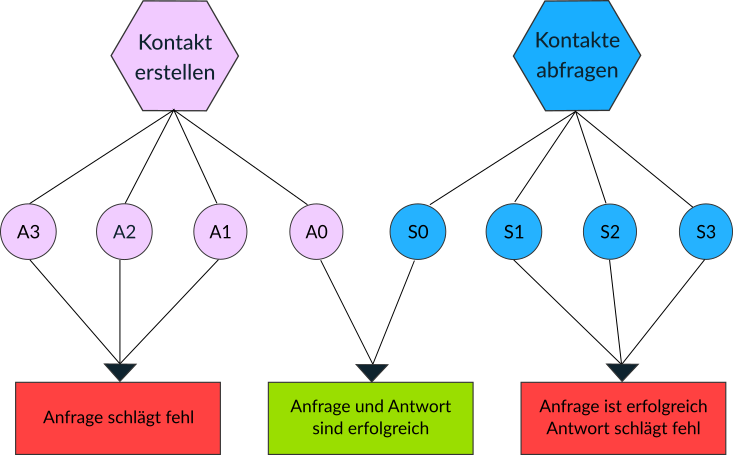
\includegraphics[width=0.8\textwidth]{Szenarien}
%   \grayRule
%   \caption[Szenarien]{Szenarien und Fälle}
%   \label{fig:scenarios}
% \end{figure}
%
% ERGEBNIS
%
\subsubsection*{Ergebnis}
Die Szenarien \it{ID0} und \it{ID1} beschreiben die Identifizierung einzelner Kontakte. Eine eindeutige Identifizierung des Kontakts ist im Szenario \it{ID0}, mittels der Verwendung einer \gls{UUID}, gewährleistet.\\
% Die Szenarien \it{V1}, \it{V2} und \it{V4}, \it{V5} beschreiben Situationen mit demselben Ausgangspunkt. In einem Fall kommt zu keinem Konflikt, in dem nächsten schon. Deswegen können \it{V1} und \it{V2}, sowie \it{V4} und \it{V5} zusammengefasst werden.
Es wird deutlich, dass es in jedem Fall zu einem Konflikt kommen kann. Es gilt zu unterscheiden in welchen Fällen mit Konflikten umgegangen werden kann und in welchen Daten verloren gehen.\\
\todo{Grafik?}\\\\
% \b{Probleme?}\\
% ID1: sprechender Schlüssel ist nicht eindeutig\\
% V0: Es kann zum Konflikt gehen weil die Version von allen Parteien gleichermaßen erhöht werden kann\\
% V1: siehe V2\\
% V2: kein Verlass auf Zeitstempel. Referenz `fallacies`?\\
% V3: ??? \highlight{logische Uhren hab ich noch nicht ganz verstanden}\\
% V4: siehe V5\\
% V5: Inhaltsbasierte Versionen sind nicht sortierbar.
%
Im weiteren Verlauf dieser Arbeit wird unter anderem beschrieben, wie diese Fälle \ldots eingebunden werden.
\todo{was passiert danach}